%%%%%%%%%%%%%%%%%%%%%%% 架构设计 %%%%%%%%%%%%%%%%%%%%%%%%%%%%%%%%%%%%%%%%%%%%%
\chapter{架构设计}

项目前端采用MVVM的软件架构,后端采用MVC的软件架构。

\section{架构描述}

\begin{enumerate}
    \item \textbf{在前端中} \\
    MVVM架构主要由四层组成,分别是Model(模型)、View(视图)和View Model(视图模型,通常包含绑定器)。
    Model层也称模型层(数据访问层),即后端数据。View层也称视图层,为前端图形用户界面。
    View Model层也称视图模型层,与视图层建立数据绑定,同时与模型层进行交互,将用户所需的数据反映成图形界面,同时将用户行为反映为后端数据变更。在本项目中,视图模型部分的功能由Vue.js提供。
    MVVM的视图模型是一个值转换器,这意味着视图模型负责从模型中暴露(转换)数据对象,以便轻松管理和呈现对象。\\
    该架构有助于将图形用户界面的开发与业务逻辑(后端逻辑)的开发分离开来。
    \item \textbf{在后端中} \\
    MVC架构主要由Model(模型)、View(视图)和Controller(控制器)组成。
    Model层也称模型层,为储存在数据库中的数据。
    View层也称视图层,直接交给前端进行处理。
    Controller层也称控制器层,负责与前端的视图模型进行交互,将后端数据同步至前端模型。
    \item \textbf{微服务架构} \\
    微服务架构是一个高度松耦合的架构,每个服务都有自己的处理和轻量通讯机制,可以部署在单个或多个服务器上。项目基于Docker微服务架构部署,将数据库、前端服务器、后端服务器封装成相对独立的Docker容器,支持即插即用,快速部署、弹性扩容,满足补充规约中对可靠性和性能的需求。
\end{enumerate}


\section{架构图}

“鲜天下”的架构设计可见\autoref{fig:mvvm}。

%\usepackage{changepage}
%\usepackage{rotating}
%\usepackage{float}
%\usepackage[section]{placeins}
%\begin{sidewaystable}[!Htp]
\begin{figure}[htp]
    %\begin{adjustwidth}{-1.5cm}{-1cm}
    \centering
    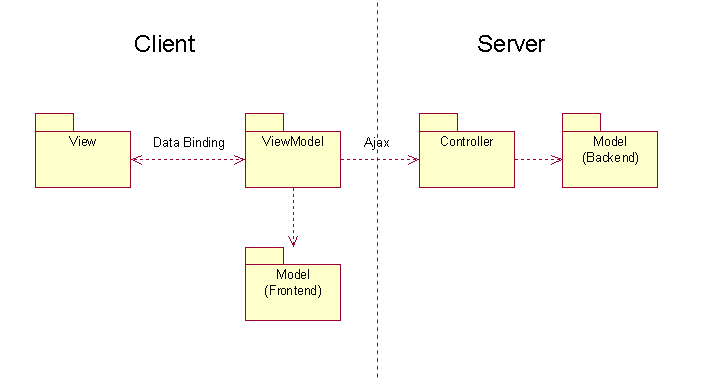
\includegraphics[width=15cm]{figure/mvvm_new.png}
    \caption{“鲜天下”-架构图}
    \label{fig:mvvm}
    %\end{adjustwidth}
\end{figure}


\section{关键抽象}

经过分析,该系统的关键抽象可见\autoref{fig:key-abstraction},本系统有如下关键实体类:

% TODO: 这个需要修正:
% 1. 删掉资金流动表
% 2. 订单表有两个,都写上去

\begin{enumerate}
    \item \textbf{用户表}:包含用户编号、用户名、密码、电子邮箱、联系方式、用户类型、余额、用户状态和钱包。
    \item \textbf{母订单}:包含订单编号、订单名称、订单概要、创建日期、截止日期、联系人地址、数量、单价、总价、创建人编号、备注、联系方式、订单状态、订单进程。
    \item \textbf{子订单}:包含订单编号、母订单编号、创建日期、创建人编号、数量、备注、联系方式、状态。
\end{enumerate}


%\usepackage{changepage}
%\usepackage{rotating}
%\usepackage{float}
%\usepackage[section]{placeins}
%\begin{sidewaystable}[!Htp]
\begin{figure}[htp]
    %\begin{adjustwidth}{-1.5cm}{-1cm}
    \centering
    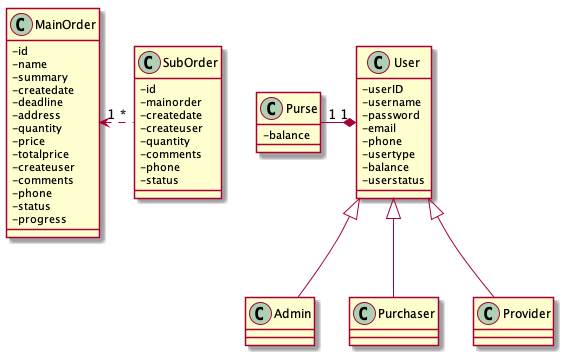
\includegraphics[width=15cm]{report/figure/key_abstract.png}
    \caption{“鲜天下”-关键抽象}
    \label{fig:key-abstraction}
    %\end{adjustwidth}
\end{figure}
